% class
\documentclass[a4paper,12pt,xelatex,ja=standard]{bxjsarticle}

% packages
%% mathematical notations
\usepackage{amsthm,amsmath,amssymb,amsfonts} % mathematical notations
\usepackage{bm} % bold character
\usepackage{latexsym} % more mathematical notations
\usepackage{physics} % physical notations
%% graphs
\usepackage{graphicx, xcolor} % graph
\usepackage{circuitikz} % for circuit elements
\usepackage{float} % positioning of graphs
\usepackage{siunitx} % SI units
\usepackage{tikz} % graphic elements
\usepackage{wrapfig} % must be after float package.
%% type system
\usepackage{bussproofs} % proof tree
%% code
\usepackage[ruled,vlined]{algorithm2e} % pseudo code
\usepackage{listings} % source code
\usepackage{inconsolata}
\lstset{
  basicstyle=\footnotesize,
  numbers=left,
  frame=single
}

% Basic information
\title{電子情報学専攻 \, 専門 \\ 令和元年 \, 解答・解説}
\author{diohabara}
\date{\today}

\begin{document}
\maketitle

\section*{第1問\ 電気・電子回路}

\subsection*{(1)}

% ref: https://jeea.or.jp/course/contents/01133/

スイッチを短絡させると、以下の回路方程式が成り立つ。

\[
  L \frac{d i(\tau)}{d \tau} = v(t)
\]

電源は定電圧電源なので \(v(t) = v(0) = E\) であり、 \(\tau = [0, t]\) 上で \(\tau\) に関して積分して整理すると

\[
  i(t) - i(0) = \frac{E}{L}t
\]

問題文より $t = 0$ で $i(0) = 0$ だから

\[
  i(t) = \frac{E}{L}t
\]

\subsection*{(2)}

スイッチを開放すると、 \(t = [T_0, T_0 + T_1)\) において以下の回路方程式が成り立つ。

\[
  L \frac{d i(t)}{d t} + \frac{1}{C}\int^{t}_{T_0}i(\tau) d \tau = E
\]

両辺を微分して整理すると

\begin{equation*}
  \begin{split}
    0 &= L \frac{d^2 i(t)}{dt^2} + \frac{1}{C}i(t) \\
    \frac{d^2 i(t)}{dt^2} &= - \frac{1}{LC} i(t)
  \end{split}
\end{equation*}

よって、\(i(t)\)の一般解は

\[
  i(t) = A \sin{\frac{1}{\sqrt{LC}}}t+ B \cos{\frac{1}{\sqrt{LC}}}t
\]

と書ける。

(1)より\(i(T_0) = \frac{E}{L}T_0\)であり\(\left.\frac{di(t)}{dt}\right|_{t=T_0}=0\)

\(\frac{di(t)}{dt} = \frac{A}{\sqrt{LC}}\cos \frac{t}{\sqrt{LC}} - \frac{B}{\sqrt{LC}} \sin \frac{t}{\sqrt{LC}}\)より

\[
  \left.\frac{di(t)}{dt}\right|_{t=T_0} = \frac{A}{\sqrt{LC}}\cos \frac{T_0}{\sqrt{LC}} - \frac{B}{\sqrt{LC}} \sin \frac{T_0}{\sqrt{LC}} = 0
\]

よって

\[
  A = B \tan \frac{T_0}{\sqrt{LC}}
\]

また

\begin{equation*}
  \begin{split}
    i(T_0)
    &= \frac{A}{\sqrt{LC}}\cos \frac{T_0}{\sqrt{LC}} - \frac{B}{\sqrt{LC}} \sin \frac{T_0}{\sqrt{LC}} \\
    &= B \left( \sin{\frac{T_0}{\sqrt{LC}}} \tan{\frac{T_0}{\sqrt{LC}}} + \cos{\frac{T_0}{\sqrt{LC}}} \right) \\
    &= B \frac{\sin^2{\frac{T_0}{\sqrt{LC}}} + \cos^2{\frac{T_0}{\sqrt{LC}}}}{\cos{\frac{T_0}{\sqrt{LC}}}} \\
    &= \frac{B}{\cos{\frac{T_0}{\sqrt{LC}}}}
  \end{split}
\end{equation*}

よって、\(i(T_0) = \frac{E}{L}T_0\)より

\begin{equation*}
  \begin{split}
    B &= \frac{E}{L}T_0 \cos{\frac{T_0}{\sqrt{LC}}} \\
    A &= B \tan{\frac{T_0}{\sqrt{LC}}} = \frac{E}{L} T_0 \sin{\frac{T_0}{\sqrt{LC}}}
  \end{split}
\end{equation*}

よって
\begin{equation*}
  \begin{split}
    i(t)
      &= \frac{E}{L} T_0 \sin{\frac{T_0}{\sqrt{LC}}} \sin{\frac{t}{LC}} + \frac{E}{L} T_0 \cos{\frac{T_0}{\sqrt{LC}}} \cos{\frac{t}{LC}}\\
      &= \frac{E}{L} T_0 \cos{\frac{1}{\sqrt{LC}}} (t - T_0)
  \end{split}
\end{equation*}

これが\(t \leq T_0\)で最初に\(0\)となるのは、\(\frac{1}{\sqrt{LC}}(t - T_0) = \frac{\pi}{2}\)のときなので

\begin{equation*}
  \begin{split}
    &\frac{1}{\sqrt{LC}}((T_0 + T_1) - T_0) = \frac{\pi}{2} \\
    &\therefore T_1 = \frac{\pi \sqrt{LC}}{2}
  \end{split}
\end{equation*}

\subsection*{(3)}

ダイオードがあるため、コンデンサにかかる電圧\(v(t)\)は常に単調増加する。\\
したがって、スイッチを開放しているときにコイルに流れる電流の時間変化

\[
  \frac{di(t)}{dt} = \frac{E - v(t)}{L}
\]

\noindent
は単調減少する。これはつまり、回数を重ねるごとにスイッチ解放後に電流が減少するスピードが早くなるということ。
だから、\(i=0\)となるまでにかかる時間は\(T_1\)からどんどん短くなっていく。\\
よって、各操作でスイッチを開放した後\(T_1\)時間後までに必ず\(i=0\)となっているはずなので、\(i(n(T_1 + T_0)) = 0\)と言える。

\subsection*{(4)}

簡単のため、\(v_k = v(k(T_0 + T_1))\)とおく。

\(k(T_0 + T_1) \leq k (T_0 + T_1) + T_0\)のとき、回路に流れる電流は(1)と同様にして

\begin{equation}
  \begin{split}
    E &= L \frac{d i(t)}{dt}, i(k(T_0 + T_1)) = 0 \\
    \therefore i(t) &= \frac{E}{L}(t - k(T_0 + T_1))
  \end{split}
\end{equation}

よって、\(t = k(T_0 + T_1) + T_0\)のとき\(i(t) = \frac{E}{L}T_0\)である。

\(k(T_0 + T_1) + T_0 \leq t < (k+1) (T_0 + T_1)\)の間について、電源がした仕事とコイル・コンデンサのエネルギーの変化分は等しいので

\[
  E \cdot C(v_{k+1} - v_k) = \left(\frac{1}{2} L \cdot 0^2 + \frac{1}{2}C v_{k+1}^2\right) +
    \left(\frac{1}{2} L (\frac{E}{L}T_0)^2 + \frac{1}{2}C v_{k}^2\right)
\]

\[
  (v_{k+1} + E)^2 = (v_k - E)^2 + \frac{E^2}{LC} {T_0}^2
\]

\(v_0 = v(0) = E\)に注意してこれを解くと

\begin{equation*}
  \begin{split}
    (v_n - E)^2 = n \cdot \frac{E^{2}}{LC}T_0^{2} \\
    \therefore v_n = E \left(1 + T_0 \sqrt{\frac{n}{LC}} \right)
  \end{split}
\end{equation*}

\section*{第2問\ 論理回路}
  \subsection*{(1)}
  AおよびBの最大値、最小値は以下の通り。
  \begin{equation*}
    \begin{split}
      A_{max} &= 0111_{(2)} = 2^3 - 1 = 7_{(10)} \\
      A_{min} &= 1000_{(2)} = -(1000 \oplus 1111 + 1)_{(2)} = -(111 + 1)_{(2)} = -8_{(10)} \\
      B_{max} &= 01_{(2)} = 2^1 - 1 = 1_{(10)} \\
      B_{min} &= 10_{(2)} = -(10 \oplus 11 + 1)_{(2)} = -(1 + 1)_{(2)} = -2_{(10)}
    \end{split}
  \end{equation*}

  \subsection*{(2)}
  半加算器、全加算器は以下のブロックとして用いる。
  \begin{figure}[H]
    \centering
    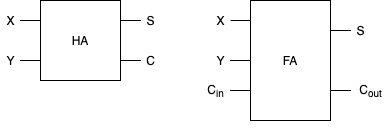
\includegraphics[width=7cm]{images/ha_and_fa.png}
  \end{figure}

  半加算器は次の通りに構成される。
  \begin{figure}[H]
    \centering
    
\includegraphics[width=5cm]{images/half_adder.png}
  \end{figure}

  全加算器は次の通りに構成される。
  \begin{figure}[H]
    \centering
    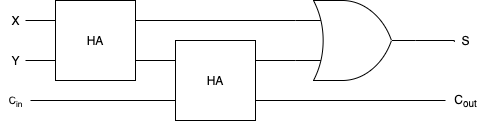
\includegraphics[width=9cm]{images/full_adder.png}
  \end{figure}

  これらを使って構成できる$A+B$を計算して$Y$を得る回路は次の通り。
  \begin{figure}[H]
    \centering
    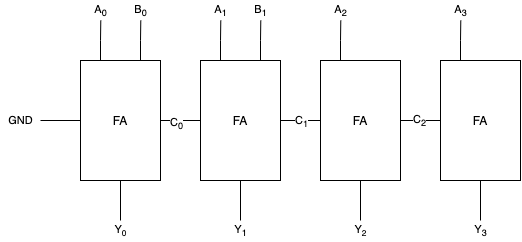
\includegraphics[width=11cm]{images/ripple_carry_adder.png}
  \end{figure}

  \subsection*{(3)}
  (2)で設計した回路がオーバフローするとき、$A_3 C_2 = 1$となる。\\
  また、(2)の回路は以下の論理式を満たす。
  \begin{equation*}
    \begin{split}
      &C_2 = A_2 C_1 \\
      &C_1 = A_1 C_0 + A_1 B_1 + B_1 C_0 = C_0(A_1 + B_1) + A_1 B_1 \\
      &C_0 = A_0 B_0
    \end{split}
  \end{equation*}
  これらの式を代入して
  \begin{equation*}
    \begin{split}
      &A_3 A_2 C_1 = 1 \\
      &A_2 A_3 (C_0(A_1 + B_1) + A_1 B_1) = 1 \\
      &A_2 A_3 (A_0 B_0(A_1 + B_1) + A_1 B_1) = 1
    \end{split}
  \end{equation*}
  よって求めるオーバフロー検知機構の回路は次の通り。
  \begin{figure}[H]
    \centering
    
\includegraphics[width=11cm]{images/overflow_detector.png}
  \end{figure}

  \subsection*{(4)}
  ビット値の符号を変換する際、それぞれの桁を反転させ$1$を加えれば良い。$A-B$を計算する際は、$A$と、$B$を反転させ1加えたものを(2)の回路で足し合わせれば良い。\\
  よって、$A-B$を計算して$Y$を得る回路は次の通り。
  \begin{figure}[H]
    \centering
    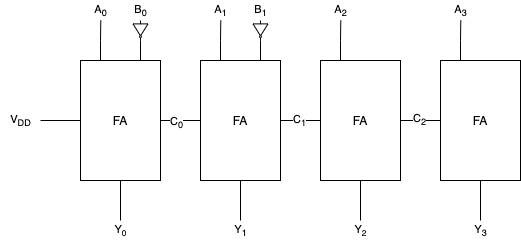
\includegraphics[width=11cm]{images/ripple_carry_subtractor.png}
  \end{figure}

  \subsection*{(5)}
  $1$ビットの信号$D$でオーバフローかどうかを出力し、オーバフロー発生時に$1$、そうでないときに$0$を出力するとする。\\
  (3)と同じように考え、$D=1$となるのは以下の論理式を満たす場合である。
  \begin{equation*}
    \begin{split}
      &A_3 C_2 = 1 \\
      &C_2 = A_2 C_1 \\
      &C_1 = C_0 (A_1 + \bar{B_1}) + A_1 \bar{B_1} \\
      &C_0 = A_0 + \bar{B_0}
    \end{split}
  \end{equation*}
  これを解いて
  \begin{equation*}
    \begin{split}
      &A_3 C_2 = 1 \\
      &A_3 A_2 C_1 = 1 \\
      &A_2 A_3 (C_0(A_1 + \bar{B_1}) + A_1 \bar{B_1}) = 1 \\
      &A_2 A_3 ((A_0 + \bar{B_0})(A_1 + \bar{B_1}) + A_1 \bar{B_1}) = 1 \\
      &A_2 A_3 (A_0A_1 + A_0 \bar{B_1} + A_1\bar{B_0} + \bar{B_0} \bar{B_1}) = 1 \\
      &A_0A_1A_2A_3 + A_0A_2A_3\bar{B_1} + A_1A_2A_3\bar{B_0} + A_2A_3\bar{B_0}\bar{B_1} = 1 \\
    \end{split}
  \end{equation*}

  以上からオーバフローが発生する入力パターンは以下の通り。ただし、*は$0$でも$1$でも良い。
  \begin{center}
    \centering
    \begin{tabular}{|l|l|l|l|l|l|}
    \hline
    $A_0$ & $A_1$ & $A_2$ & $A_3$ & $B_0$ & $B_1$ \\ \hline \hline
    1  & 1  & 1  & 1  & *  & *  \\ \hline
    1  & *  & 1  & 1  & *  & 0  \\ \hline
    *  & 1  & 1  & 1  & 0  & *  \\ \hline
    0  & 0  & 1  & 1  & 0  & 0  \\ \hline
    *  & 1  & 1  & 1  & *  & 0  \\ \hline
    \end{tabular}
  \end{center}

\section*{第3問\ アルゴリズム}
  \subsection*{(1)}
  \begin{lstlisting}
    if CONTAIN-INTEGERS(M, A, i, j) and (j - i <= end - start):
        start = i
        end = j
  \end{lstlisting}
  擬似コードの説明をする。\\
  CONTAIN-INTEGERS(M, A, i, j)は条件を満たす部分配列かどうかを確認している。今for文内で調べている部分配列の長さは$j-i$であり、現在最短の部分配列の長さは$end-start$である。そのため、$j-i \leq end-start$を満たせば良い。これが2つ目の条件式である。\\
  これらを満たす部分配列は最短かつ開始位置が最大であるから、startとendを更新する。

  \subsection*{(2)}
  手元で確認すると以下のような結果となる。
  \begin{center}
    \centering
    \begin{tabular}{|l|l|l|l|l|}
    \hline
    i & j & $A^{end}_{start}$ & start & end \\ \hline \hline
    0 & 1 & <1, 1, 0, 1>    & 0     & 4   \\ \hline
    0 & 2 & <1, 1, 0, 1>    & 0     & 3   \\ \hline
    0 & 3 & <1, 1, 0>       & 0     & 3   \\ \hline
    0 & 4 & <1, 1, 0>       & 0     & 3   \\ \hline
    1 & 2 & <1, 1, 0>       & 0     & 3   \\ \hline
    1 & 3 & <1, 0>          & 1     & 3   \\ \hline
    1 & 4 & <1, 0>          & 1     & 3   \\ \hline
    2 & 3 & <1, 0>          & 1     & 3   \\ \hline
    2 & 4 & <0, 1>          & 2     & 4   \\ \hline
    3 & 4 & <0, 1>          & 2     & 4   \\ \hline
    \end{tabular}
  \end{center}

  \subsection*{(3)}
  \begin{lstlisting}[mathescape]
  FIND-SNIPPET(N, M, A):
      start = 0
      end = N
      j = 1
      for i = 0 to N-1 do
          while j - i <= 0 or (j < N and not CONTAIN-INTEGERS(M, A, i, j)):
              j += 1
          if CONTAIN-INTEGERS(M, A, i, j) and j - i <= end - start:
              start = i
              end = j
      return $A^{end}_{start}$
  \end{lstlisting}
  擬似コードの説明をする。\\
  two pointers techniqueを使う。for文で部分配列の左端を右にずらしていく。\\
  while文では部分配列の右端をずらしている。最初の条件は部分配列の長さが0以下、つまり部分配列が存在しないことを意味し、このときに右端を伸ばして部分配列の長さが1以上となるようにする。
  次の条件式はjが配列Aの右端でなく、問題の条件を満たさないことを意味する。よってこれは部分配列が問題の条件を満たすまで右端を伸ばすということ。
  最後の条件式は(1)同様のもので、これで最短部分配列が求められることはわかった。\\
  次にこの計算量が$O(N)$になることを説明する。\\
  iは0からN-1まで移動し、jは1からNまで移動する。(1)のアルゴリズムと異なり、iもjも単調増加であり、i+jは一意となるので最大でも$N+N=2N$回のステップしか動作はしない。それぞれのステップで必要な計算は$O(1)$だから、全体で$O(N)$で動作する。

  \subsection*{(4)}
  区間$[i, j]$で使われていない数を保持するスタックunusedと区間$[i, j]$に含まれる数の個数を保持する配列countを用意する。ただし、添字が数、値がその個数とする。\\
  unusedを$\{0, 1, \dots, M-1\}$で初期化し、countはすべての要素を$0$で初期化する。\\
  CONTAIN-INTEGERSは以下のような関数とする。
  \begin{lstlisting}
  CONTAIN-INTEGERS(M, A, i, j):
      while stack:
          number = stack.top()
          if 0 < count[number]:
              stack.pop()
          else:
              return False
      return True
  \end{lstlisting}
  そして、iが右にずれるとき
  \begin{lstlisting}
    count[A[i]] -= 1
    stack.push(A[i])
  \end{lstlisting}
  jが右にずれるとき
  \begin{lstlisting}
    count[A[j]] += 1
  \end{lstlisting}
  と処理する。この処理は各ステップが$O(1)$であり、CONTAIN-INTEGERSの処理も全体でO(N)回しか行われず、ならし計算量は$O(1)$となる。

\section*{第4問\ ネットワーク}
  \subsection*{(1)}
  \subsection*{(2)}
  \subsection*{(3)}
  \subsection*{(4)}
  \subsection*{(5)}
    \subsubsection*{(a)}
    \subsubsection*{(b)}

\section*{第5問\ 情報理論}
  \subsection*{(1)}
  \subsection*{(2)}
  \subsection*{(3)}
  \subsection*{(4)}
  \subsection*{(5)}
  \subsection*{(6)}
  \subsection*{(7)}

\end{document}

